\newpage
\section{Praktische Umsetzung} \label{sec_praktische_umsetzung}

In der praktischen Umsetzung werden die Grundlagen auf den Anwendungsfall angewendet. Hierfür wird zunächst der \ac{OSMI}-Index erläutert.
Es folgen die Bildklassifizierung und die Umsetzung der \acf{NER}. Zum Abschluss des praktischen Teils folgt ein Kapitel
mit Consultinganteil.

\subsection{OSMI-Index} \label{subsec_osmi}

\begin{figure}[H]
	\caption{Zielbild des Consulting-Projekts}\label{fig:zielbild}
	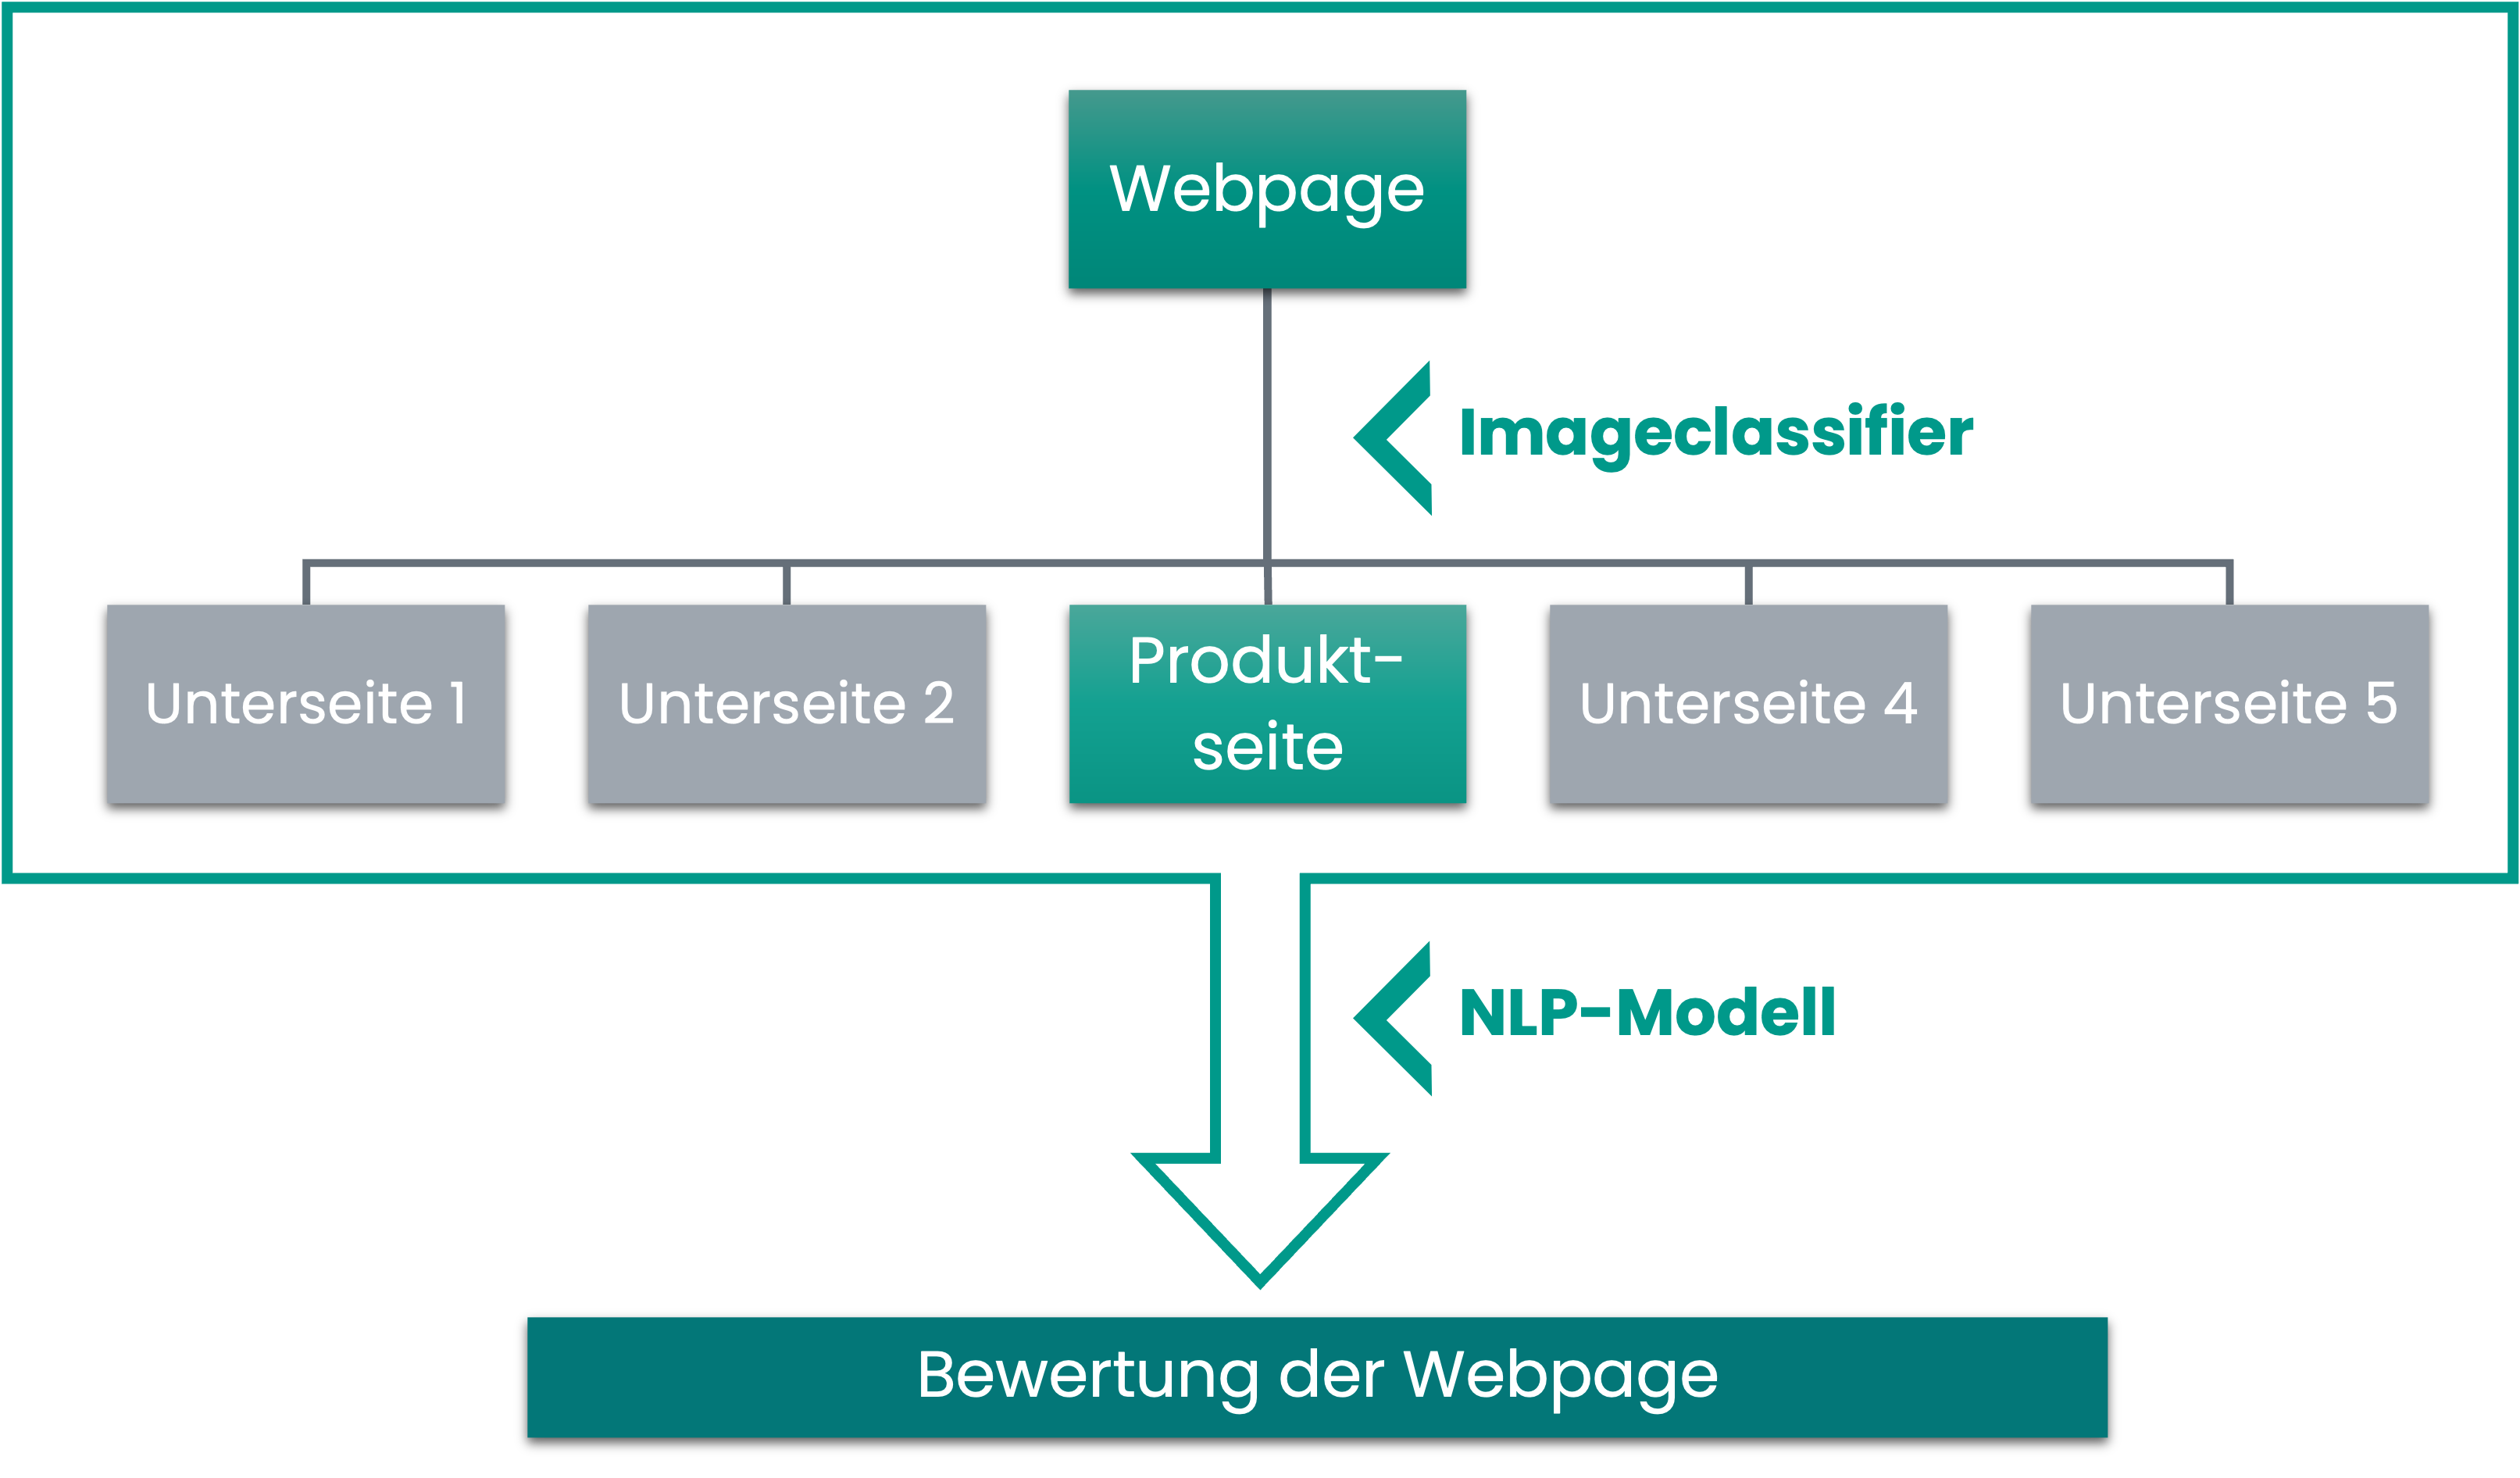
\includegraphics[width=0.9\textwidth]{zielbild.png}
	\\
	Quelle: Eigene Darstellung
\end{figure}

Um den OSMI-Index zu optimieren und zu automatisieren wurde die in Abbildung~\ref{fig:zielbild} Pipeline aufgestellt mithilfe dessen
eine Website in Bezug auf den OSMI verarbeitet wird.
Der erste Schritt stellt dabei eine Vorverarbeitung der zu analysierenden Website dar, indem ein Image Classifier die Haupt- und Unterseiten der Website in
Produkt- und Nicht-Produktseiten unterteilt.
Dies ist aus Sicht der Autoren dieser Hausarbeit ein essenzieller Schritt, da so sichergestellt wird, dass die Bewertung des OSMI-Index lediglich auf Basis
der relevanten URLs vorgenommen wird.
Im darauf folgenden Schritt wird auf die textlichen Inhalte der relevanten Produktseiten ein \ac{NLP}-Modell angewendet, welches die Entitäten des OSMI-Index erkennt und auszählt.
Im abschließenden Schritt werden die Ergebnisse der Website-Analyse im Rahmen eines Dashboards visualisiert.
Nachfolgend wird die Umsetzung der soeben beschriebenen Schritte im Detail beschrieben und erläutert.

\subsection{Datenvorbereitung}

Sowohl in der Literatur als auch in bereits etablierten, gut entwickelten und veröffentlichten Modellen ist das Gebiet
des Sensory Marketings sehr rar vertreten.
Das bedeutet auch, dass im Hinblick auf den jüngst publizierten \ac{OSMI}-Index ebenfalls bisher wenig technische Entwicklungen
vorgenommen worden sind.
Zwar existieren in der Literatur diverse NLP-Modelle wie beispielsweise das generelle Spacy-Modell oder der sogenannte BERT
und von beiden erwähnten Modellen Spezialisierungen wie beispielsweise SciSpacy, BioBERT, ESG-BERT, etc\., allerdings ist
bisher kein NLP-Modell auf Marketingkontexte trainiert und publiziert worden, sodass die Notwendigkeit zur Entwicklung eines
eigenen Modells im Kontext des Consulting-Auftrags bestand.
Um im Vorfeld der Website-Bewertung jedoch lediglich nur die relevanten URLs mit Produktinhalt zu selektieren, wurde für den zu
entwickelnden Image Classifier ebenfalls ein von Grund auf neu zu entwickelndes Modell benötigt, da es innerhalb der Literatur
bislang kein derartig existierendes Modell publiziert wurde auf das zurückgegriffen werden konnte.

Die Trainingsdaten wurden mithilfe von Doccano generiert.
Doccano ist ein open source Tool, welches zur Annotation von Text und Bilddaten entwickelt wurde.
Mit diesem Instrument ist es also möglich Textpassagen und Bilder hochzuladen und Annotationen vorzunehmen, um Daten zur
Entwicklung von Aufträgen wie Named-Entity-Recognition, Textzusammenfassungen, Sentimentanalysen, Image Classification, etc.
zu generieren.

Im Rahmen des Consulting-Projekts wurden zwei Doccano-Projekte gestartet.
Ein Projekt wurde für das Annotieren von Textpassagen zur Entwicklung eines Named-Entity-Recognition Modells erstellt.
Im zweiten Projekt wurden Screenshots von Produktseiten und Nicht-Produktseiten annotiert.

Die Textpassagen, die annotiert wurden, sind im Rahmen des Consulting-Projekts zur Verfügung gestellt worden und entstammen
Webscraping-Ergebnissen von Vorgängerprojekten.
Hier wurden die fünf Sinne
\begin{itemize}
	\item Sight
	\item Smell
	\item Sound
	\item Taste
	\item Touch
\end{itemize}
als Label festgelegt und konnten im Rahmen des Annotationsprozesses ausgewählt werden.
Die in Abbildung~\ref{fig:annotation_ner} dargestellten horizontalen Balken geben den Annotationsstand wieder, auf Basis dessen
das Modell zur Erkennung von Entitäten entwickelt wurde.
Hier ist zu erkennen, dass die Entität \glqq{Sight}\grqq am häufigsten annotiert worden ist, während die Trainigs- und Testdaten für
die Entität \glqq{Smell}\grqq, \glqq{Sound}\grqq sowie \glqq{Taste}\grqq kaum vertreten sind.
\begin{figure}[H]
	\caption{Annotationsstand Textlabeling}\label{fig:annotation_ner}
	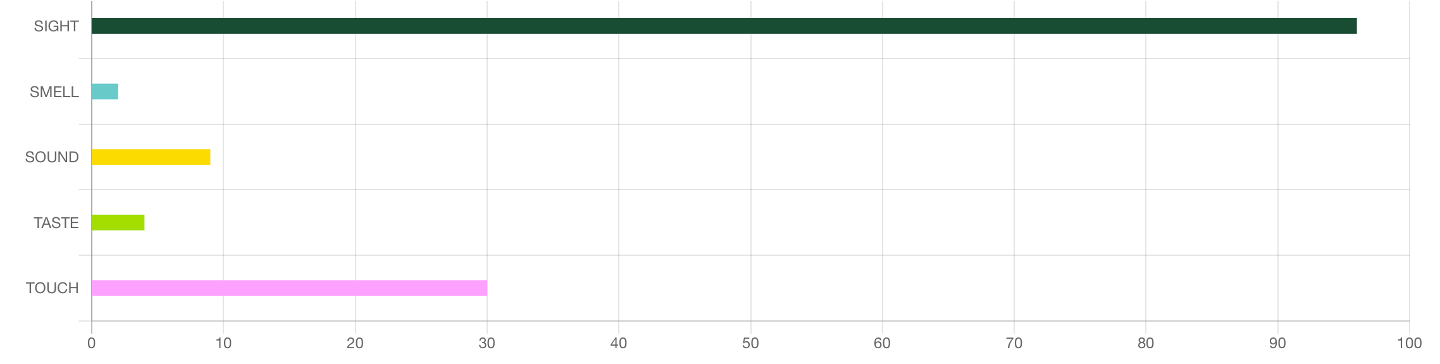
\includegraphics[width=0.9\textwidth]{annotationen_ner.png}
	\\
	Quelle: Eigene Darstellung
\end{figure}
Die zu annotierenden Bilddaten von Produkt- und Nicht-Produktseiten wurden im Rahmen des behandelten Projektes selbständig
generiert.
Abbildung~\ref{fig:annotation_imgclf} zeigt, dass zur Modellentwicklung für den Image Classifier eine fast Gleichverteilung zwischen Produkt-
und Nicht-Produktseiten zugrunde gelegt wird.
Der Gesamtdatensatz beläuft sich auf rund 500 annotierten Bildern von Homepages.
\begin{figure}[H]
	\caption{Annotationsstand Textlabeling}\label{fig:annotation_imgclf}
	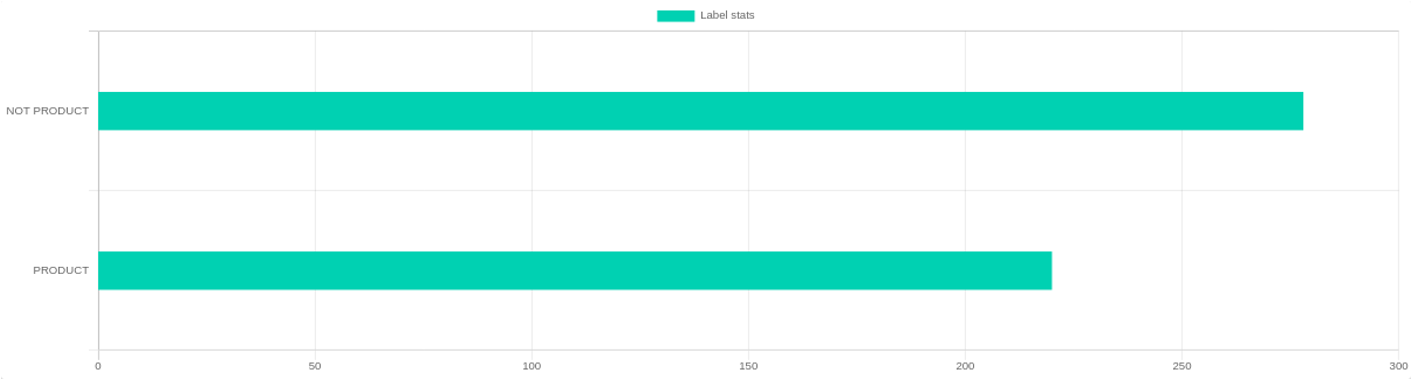
\includegraphics[width=0.9\textwidth]{annotationen_imgclf.png}
	\\
	Quelle: Eigene Darstellung
\end{figure}

-Gewichtung der Indikatoren wird im \ac{OSMI} nicht vorgenommen, weil nicht zweifelsfrei zu
argumentieren welcher mehr oder weniger bewertet wird (bisher keine Forschungsarbeiten
dazu) \\
-Indikatoren werden einzeln bewertet \& letztendlich fünf Parameter zw. 0 \& 1 liegen vor.
Daraus ergibt sich Gesamt-Index (ohne Gewichtung, arithmetischer Durchschnitt) für jede
Webseite > auch zw. 0 \& 1 und ist dann der \ac{OSMI}-Index \\
-Je näher der \ac{OSMI} an einer 1, desto erfolgreicher spricht die Webseite die Sensorik an. Wert
nahe 0 erhält wichtige Elemente entsprechend nicht \& erfüllt die Indikatoren nicht \\
-BSP eines \ac{OSMI}-Indexes: Bild einfügen aus der Masterarbeit mymuesli.de oder so



möglicher Aufbau:
1.	Bildklassifizierung
	a.Datenset
	b.Umsetzung
2.	NER
	a.	Datenset
	b.	Umsetzung
3.	Zusammenführung
4.	Consultingteil

\subsection{Klassifizierung von Webseiten} \label{subsec_klassifierung_websites}
Zur Differenzierung von Produkt- und nicht-Produkt Webseiten soll ein Klassifizierungsmodell erstellt werden.
Im Folgenden wird das Vorgehen mit den Schritten der Datenerhebung (\ref{subsubsec_class_datenerhebung}), der Datenverarbeitung (\ref{subsubsec_class_datenverarbeitung}) und des Modelltrainings (\ref{subsubsec_class_training}) näher beschrieben.
\subsubsection{Datenerhebung} \label{subsubsec_class_datenerhebung}
Aus vergangenen Arbeiten von Studierenden steht bereits eine Datengrundlage zur Verfügung mit Textauszügen, dem HTML Quelltext und heruntergeladenen Bildern von Unternehmenswebseiten.
Für die Klassifizierung werden jedoch Bilder beziehungsweise Screenshots benötigt, die die gerenderte, visuelle Struktur der Webseite erfassen.
Dies ist in den bestehenden Daten nicht gegeben und macht daher eine erneute Erhebung notwendig.

Für diesen Zweck wurde zunächst ein Webcrawler auf Basis von Scrapy \footcite[\vglf][]{zotero-328} erstellt, der alle in der Vergangenheit gescrapten Webseiten aufruft und einen Screenshot der jeweiligen Seite erstellt.
Auf diese Weise wurden circa 10.000 Bilder gesammelt, die als Eingangsdaten für das Modell verwendet werden können.

\begin{figure}[H]
    \centering
    \caption[]{Bildklassifizierung in Doccano}
	\label{fig:doccano_products}
    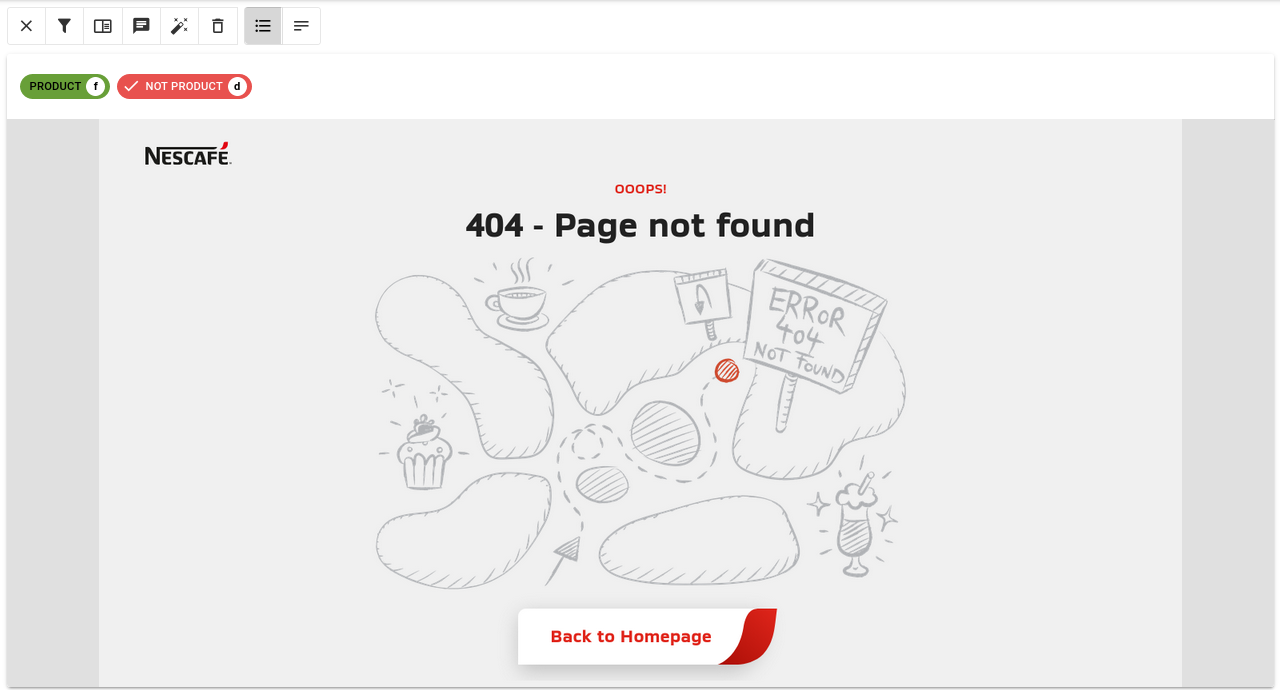
\includegraphics[width=1\textwidth]{doccano_product_annotation.png}
\end{figure}
Da es sich bei der Klassifizierung um eine Supervised Learning Methode handelt, müssen die Daten daraufhin den Kategorien \textit{Product} und \textit{Non Product} zugeordnet werden.
Dafür werden die Daten in die Annotationssoftware Doccano\footcite[\vglf][]{doccano-2018} geladen und dann, wie in Abbildung \ref{fig:doccano_products} dargestellt, den Kategorien zugeordnet.

\subsubsection{Datenverarbeitung} \label{subsubsec_class_datenverarbeitung}
Im Schritt der Datenverarbeitung werden die Eingangsdaten in eine Form gebracht, in der sie für das Training des Modells verwendet werden können.
Dazu werden die Bilder anhand des Exports der Annotationen aus Doccano in den Labeln gleichnamige Ordner verschoben.

Da die Screenshots als \textit{.png} Bilder vorliegen, verfügen sie über einen Alpha-Channel der für die Verwendung im Modell hinderlich ist.
Aus diesem Grund wurde dieser in einem weiteren Schritt entfernt.
Darüber hinaus werden die Bilder im ersten Layer des Modells auf eine Größe von 224x224 Pixeln herunterskaliert, was eine gängige Größe für \aclp{CNN} darstellt.\footcite[\vglf][\pagef 79]{ghosh2019}


\subsubsection{Training des Modells} \label{subsubsec_class_training}
Nachdem die Daten, wie in Kapitel \ref{subsubsec_class_datenverarbeitung} beschrieben, verarbeitet wurden, können Sie im weiteren Verlauf für das Training eines Modells verwendet werden.
Dazu wurden die Daten wie im Deep Learning üblich, in Train und Validation Sets aufgeteilt um einen späteren Vergleich auf unbekannten Daten zu ermöglichen.
\begin{figure}[!h]
    \centering
    \begin{subfigure}[b]{0.49\textwidth}
        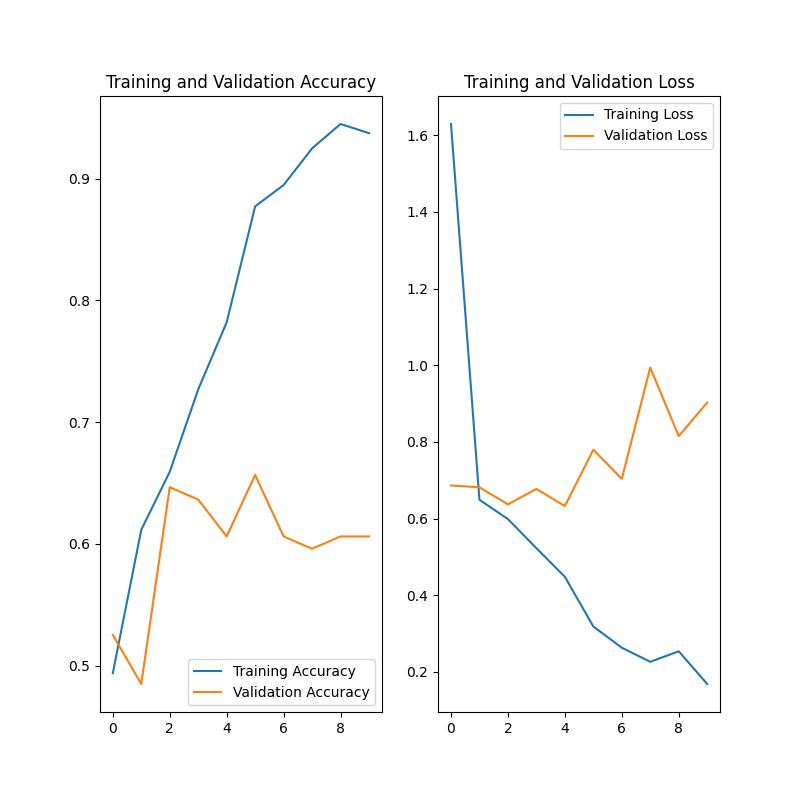
\includegraphics[width=\textwidth]{abbildungen/acc_train_val.png}
        \caption {Accuracy}
        \label{fig:metricsTrainAcc}
    \end{subfigure}
    \begin{subfigure}[b]{0.49\textwidth}
        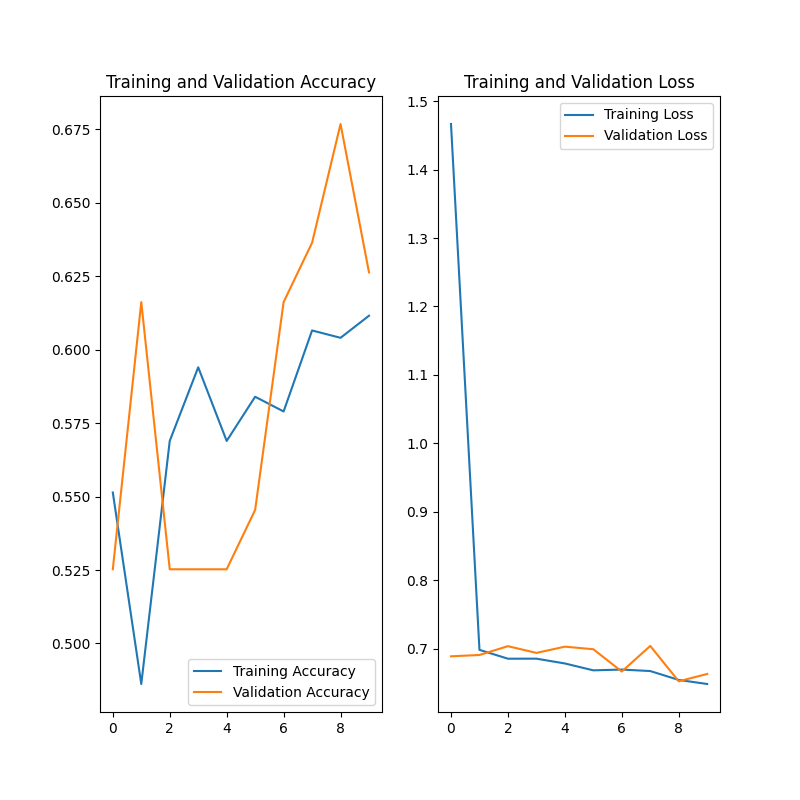
\includegraphics[width=\textwidth]{abbildungen/loss_train_val.png}
        \caption {Loss}
        \label{fig:metricsTrainLoss}
    \end{subfigure}
    \caption {Vergleich der Trainings- und Validierungsmetriken}
    \label{fig:metricsTrain}
    \textit{Quelle: Eigene Darstellung}
    \\
\end{figure}
Abbildung \ref{fig:metricsTrain} stellt jeweils die Trainings- und Validierungsmetriken für die \textit{Accuracy} und den \textit{Loss} gegenüber.
Es ist erkennbar, dass die Graphen in beiden Abbildungen relativ früh auseinander gehen, was darauf hindeutet, dass ...
Insgesamt muss gesagt werden, dass die erzielten Genauigkeiten und Losses weit von einem idealen Ergebnis entfernt liegen.
